
\section{Benutzerhandbuch}

\subsection{Projektauswahlfenster}
Das Programm startet mit einem Auswahlfenster für Projekte. Hier haben Sie die Möglichkeit zuletzt erstellte Projekte zu öffnen, andere existierende Projekte hinzuzufügen oder ein neues Projekt zu erstellen. 

\begin{figure}[h!]
	\centering
	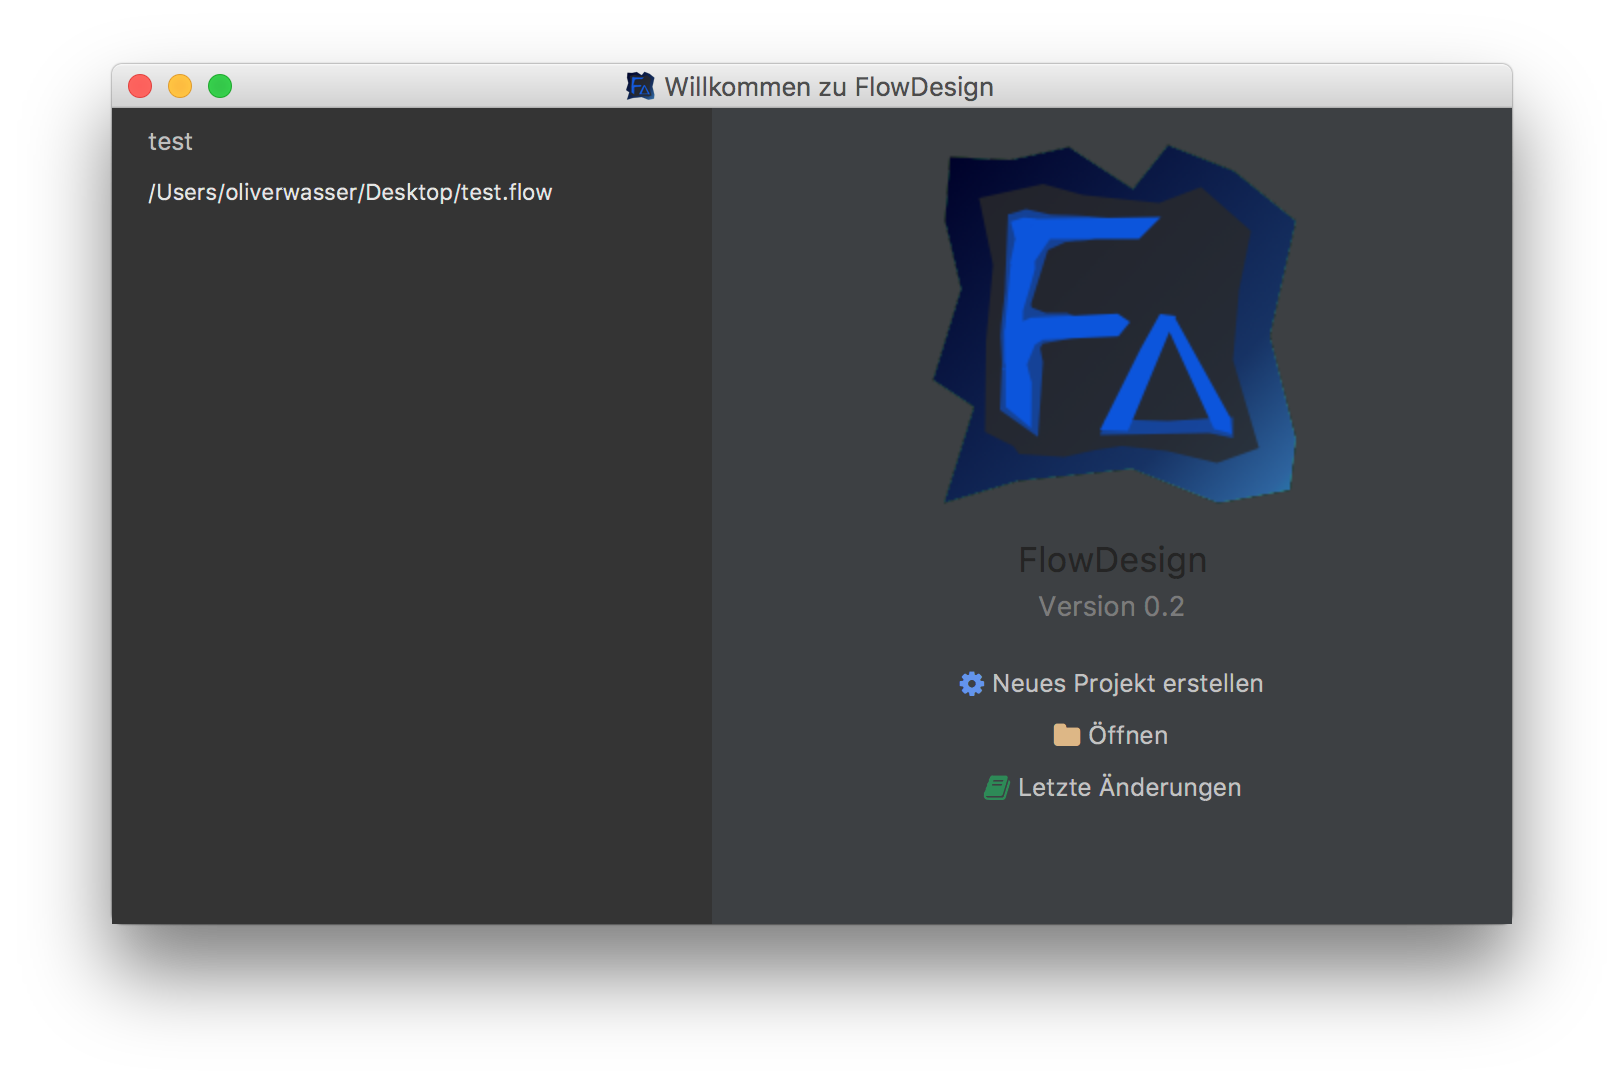
\includegraphics[width=1.0\textwidth]{Auswahlfenster.png}
	\caption{Auswahlfenster}
\end{figure}

\begin{itemize}
\item Zum Öffnen eines kürzlich erstellten Projekts, wählen Sie mit einem Doppelklick das gewünschte Projekt im linken Teil des Auswahlfensters. 
\item Zum Hinzufügen eines anderen bestehenden Projektes, wählen Sie mit einem Linksklick ''Öffnen''. Es erscheint ein Fenster zur Auswahl des Dateipfades. Wählen Sie nun das gewünschte Projekt als ''.flow'' Datei aus und bestätigen Sie anschließend mit ''Open''. 
\item Zum Erstellen eines neuen Projektes, drücken Sie "Neues Projekt erstellen". Im folgenden Fenster tragen Sie einen Name und Speicherort für Ihr Projekt ein. Bestätigen Sie mit ''Ok''.  
\end{itemize}



\subsection{Projektfenster}
\subsubsection{Menüleiste}
\subsubsection{Projektbaum}
\subsubsection{Zeichenfläche}
